%************************************************
\chapter{Results}\label{ch:results}
%************************************************
In this chapter, the learning performance and regularization behavior of the ALIF, STDP-ALIF, and Izhikevich neurons are compared.
Then, the effect of stacking multiple recurrent layers on the learning performance and speed is examined.

\section{Comparing neuron models}
	\paragraph{Accuracy}
		The main result of this report is that the STDP-ALIF and Izhikevich neuron models result in faster convergence.\todo{recheck and finish, reference each subfig individually and describe.}

		\begin{figure}[bth]
		    \myfloatalign
		    \subfloat[Percentage of samples wrongly classified.]
		    {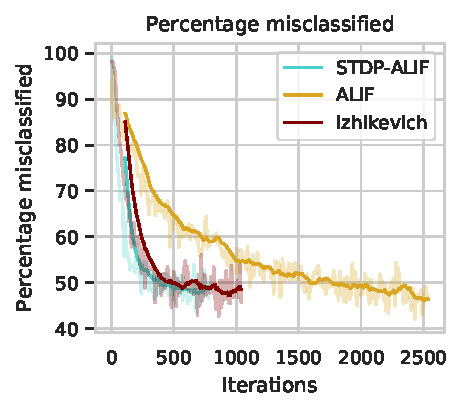
\includegraphics[width=.45\linewidth]{gfx/percwrong}} \quad
		    \subfloat[Cross-entropy loss (log-scaled).]
		    {\label{fig:crossentropy}%
		        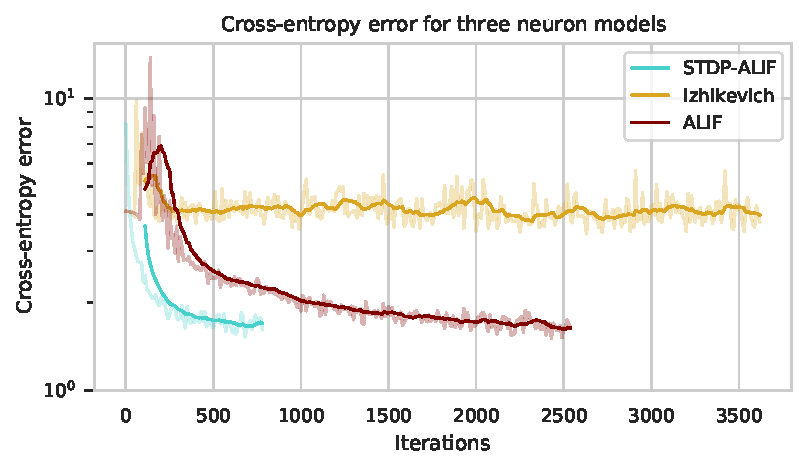
\includegraphics[width=.45\linewidth]{gfx/crossentropy}}
		    \caption[Classification performance for each of the three neuron models in a single-layer e-prop model.]{Classification performance on the validation data for each of the three neuron models in a single-layer e-prop model.}\label{fig:sl-acc}
		\end{figure}

	\paragraph{Firing rate}
		\begin{figure}[bth]
		    \myfloatalign
		    \subfloat[Mean spiking frequency.]
		    {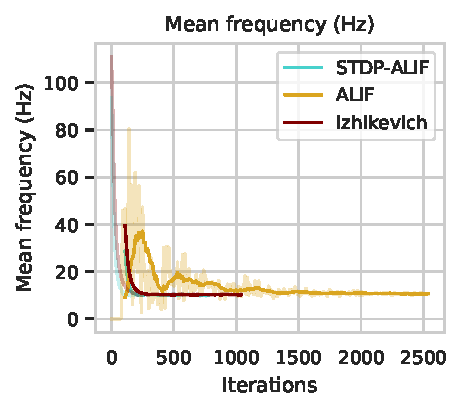
\includegraphics[width=.45\linewidth]{gfx/hz}} \quad
		    \subfloat[Regularization error.]
		    {\label{fig:regerr}%
		        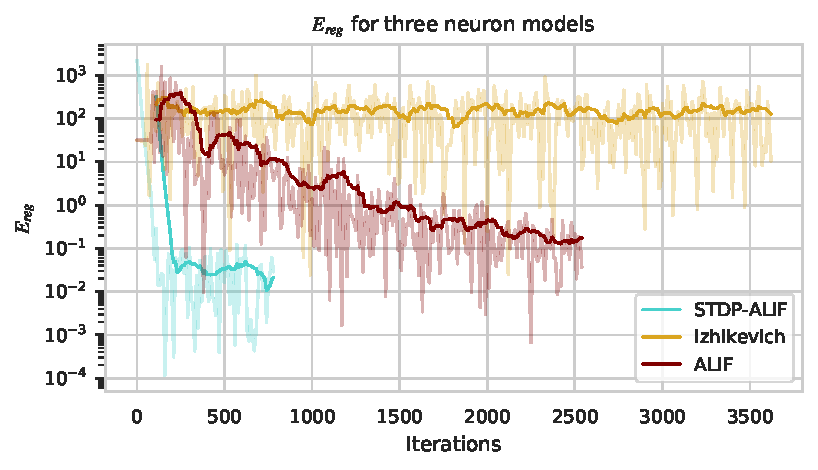
\includegraphics[width=.45\linewidth]{gfx/regerr}}
		    \caption[Effect of firing rate regularization for each of the three neuron models.]{Effect of firing rate regularization on the validation data for each of the three neuron models.}\label{fig:sl-reg}
		\end{figure}

\section{Comparing network depth}
From the comparison between the network depth, it can be concluded that XYZ\todo{write this}

\begin{figure}[bth]
    \myfloatalign
    \subfloat[ALIF model.]
    {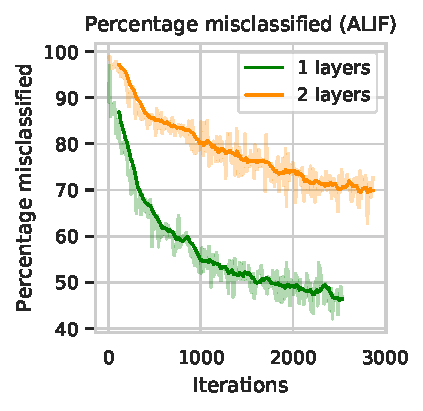
\includegraphics[width=.45\linewidth]{gfx/ml-percwrong-ALIF}} \quad
    \subfloat[STDP-ALIF model.]
    {\label{fig:pwrong_alif}%
        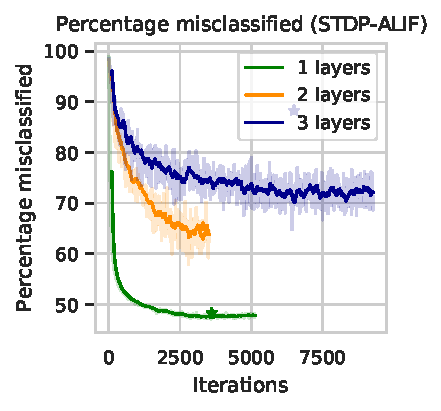
\includegraphics[width=.45\linewidth]{gfx/ml-percwrong-STDP-ALIF}} \\
    \subfloat[Izhikevich model.]
    {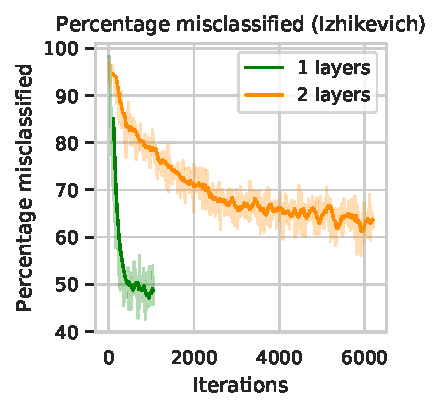
\includegraphics[width=.45\linewidth]{gfx/ml-percwrong-Izhikevich}}
    \caption[Single- and multi-layer accuracy comparison]{Accuracy comparison on the validation data between single- and multi-layer e-prop models.}\label{fig:ml-percwrong}
\end{figure}
